\documentclass[12pt]{article}
%Gummi|065|=)
\usepackage{amsmath, amsfonts, amssymb}
\usepackage[margin=0.5in]{geometry}
\usepackage{xcolor}
\usepackage{graphicx}
%\usepackage{graphicx}
\newcommand{\off}[1]{}
\DeclareMathSizes{20}{30}{21}{18}

\newcommand{\myhrule}{}

\newcommand{\two }{\sqrt[3]{2}}
\newcommand{\four}{\sqrt[3]{4}}

\newcommand{\dash}{
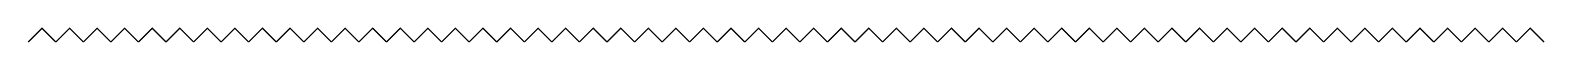
\begin{tikzpicture}[scale=0.35]
\foreach \x in {1,...,55}{
	\draw (\x,-0.25)--(\x+0.5,0.25)--(\x+1,-0.25);
}
\end{tikzpicture}
}

\newcommand{\sq}[3]{
\node at (#1+0.5,#2+0.5) {#3};
\draw (#1+0,#2+0)--(#1+1,#2+0)--(#1+1,#2+1)--(#1+0,#2+1)--cycle;
}

\usepackage{tikz}

\title{\textbf{Prime Number Theorem}}
\author{John D Mangual}
\date{}
\begin{document}

\fontfamily{qag}\selectfont \fontsize{25}{30}\selectfont

\maketitle

\noindent The Wiener-Ikehera Tauberian Theorem implies the Prime Number Theorem, as can be shown in various places. \\ \\ None of those discussions really explain to me:
\begin{itemize}
\item connection to divergent series
\item how we can proceed on our own
\end{itemize}
Norber Weiner's original argument is very easy to follow:
M\"{o}bius inversion is what gives the series to start:
$$ \sum_{m=1}^\infty x^m \log m = \sum_{n=1}^\infty \Lambda(n) \frac{x^n}{1-x^n} $$
and then set $x = e^{-\xi}$ and $\xi \to 0$ (or $x \to 1$). \newpage

\noindent
The two limiting behaviors are rather diffrent
$$  \frac{x^n}{1 - x^n}  = \left\{  \begin{array}{rl}
1/n\epsilon & \text{ as }x \to 1 \\
\epsilon^n & \text{ as } x \to 0 \end{array}\right. $$
and the cuttoff point is when $(1 - \epsilon)^n$ is getting small (near $n = 1/\epsilon$)
$$ \sum_{n=1}^\infty \Lambda(n) \frac{\xi e^{-n\xi}}{1-e^{-n\xi}} \approx \sum_{n=1}^{1/\xi} \frac{\Lambda(n)}{n} $$
Maybe if we take the derivative of both sides:
$$  \sum_{n=1}^\infty \Lambda(n) \; \frac{d}{d(n\xi)}\bigg[ \frac{n\xi }{1-e^{n\xi}} \bigg]  \approx \sum_{n=1}^{1/\xi} \Lambda(n) $$
 And clearly the two sides are approximate so we are done.
$$ \frac{d}{du} \left( \frac{u}{1 - e^u} \right) = \left\{  \begin{array}{cl}
1 & \text{ as }u \to 0 \\
ue^{-u} & \text{ as } u \to \infty \end{array}\right. $$
The left side can be shown to be 1 through ``elementary" arguments. 
$$  \sum_{n=1}^\infty \Lambda(n) \; \frac{d}{d(n\xi)}\bigg[ \frac{n\xi }{1-e^{n\xi}} \bigg] \approx \frac{1}{\xi} + O(\log \xi)$$

\newpage

\fontfamily{qag}\selectfont \fontsize{12}{10}\selectfont


\begin{thebibliography}{}

\item David Vernon Widder \textbf{The Laplace Transform} Princeton University Press, 1948.

\item Norbert Wiener \textbf{Tauberian Theorems} Annals of Mathematics Vol. 33, No. 1 , pp. 1-100

\item G. H. Hardy \textbf{Divergent Series} Oxford University Press 1973

\end{thebibliography}

\newpage

\fontfamily{qag}\selectfont \fontsize{25}{30}\selectfont

\noindent The argument in the previous section is wrong.\footnote{I got really good at writing glib and suggestive proofs to hand in to graders.  Who themselves are not always sure so they give you a check.
$$ \sum^{1/\xi}_{n=1} a_n \, g( n \epsilon) \approx \sum^{1/\xi}_{n=1} a_n g(0) $$
Glib arguments can be acceptable, since we don't always have the time / resources to check all the cases.}  \\ \\It is very difficult to express in a vivid way - with images - why it is incorrect.  \\ \\
And in most situations it doesn't really matter. As for motivation, I can only speak for myself. \\
\begin{itemize}
\item why is Prime Number Theorem in a book on Laplace Transforms?
\item why is Prime Number Theorem in a book in Divergent Series? \\
\end{itemize}
These lead me to neo-classical approaches - they will feel pretty modern to you!\footnote{I tried to read the most modern papers first: there is Tao and Gowers and Green.  However, that conversation pre-supposes knowledge I don't have and is written in language that I really don't like.  They are pretty dreadful to read as are most papers in Analytic Number Theory as well as the people who write them!y  The ``beauty of the primes" is just a marketing term.} \\ \\
One possibility is: \textbf{there is nothing new under the sun}.  Everything is thinly dressed-up versions of the same problems since antiquity.
\newpage

\noindent And that's pretty much how we feel.  So let's try take some examples from \texttt{hep-th} and \texttt{math-nt}. \\ \\
Hopefully, also finish a real proof of PNT.\footnote{The terms ``combinatorial" or ``geometric" or ``algebraic" or ``elementary" have all been misleading and so I have often chosen to start from scratch.}  What could possibly go wrong with approximations like this? 
$$ \sum_{n=1}^\infty \Lambda(n) \frac{\xi e^{-n\xi}}{1-e^{-n\xi}} \approx \sum_{n=1}^{1/\xi} \frac{\Lambda(n)}{n} $$
Maybe if we take the derivative of both sides:
$$  \sum_{n=1}^\infty \Lambda(n) \; \frac{d}{d(n\xi)}\bigg[ \frac{n\xi }{1-e^{n\xi}} \bigg]  \approx \sum_{n=1}^{1/\xi} \Lambda(n) $$
These should be satisfactory in any Physics or Engineering textbook. 

\newpage 

\noindent By default plotting the van Mandolt function uses \textbf{linear interpolation} - disastrous.

\includegraphics{vanmangoldt-01.png}  

\noindent If we use ``dots" we get that $\Lambda(n)$ has two parts $\Lambda(n) = 0$ when $n \neq p^k$ a prime power, and also $\Lambda(n) = \log p$ when $n = p^k$.  Mysterious\footnote{It is related to $\zeta'(s)/\zeta(s)= \sum \frac{\Lambda(n)}{n^s}$.}\\
\includegraphics{vanmangoldt-02.png} 

\newpage

\noindent The cumulative sum\footnote{basically adding all the numbers.  Please observe that $e^{\sum_{n \leq x} \Lambda(n)} = \mathrm{lcm}(1,2,\dot, n) \approx e^x$. This is another way of stating PNT.  The Least Common Multiple and the Permutation Group should play a more central role! } $\sum_{n \leq x} \Lambda(n) \approx x$ we get almost a straight line. For comparison $y=x$.

\includegraphics{vanmangoldt-03.png}  

\noindent The blue curve was consistently above the line in our range.  This bias in an artifact of our choice primes $1 < p < 10^3$

\includegraphics{vanmangoldt-04.png}  

\newpage

\noindent These pictures what the statement of PNT could mean:
$$ \sum_{n \leq x} \Lambda(n) \approx x + o(x)$$
Sometimes when reading a complicated passage I'd get cynical:\footnote{My latest idea is that Prime Number Theorem summarizes experiences with prime numbers up to a certain level.  If you're not a cryptographer, it is possible that prime number theory or the zeta function plays an implicit level.}
\begin{itemize}
\item why prime numbers?
\item where do we consider averages over primes?
\item why does it get so difficult? 
\end{itemize}
The tools and arguments get increasingly sophicistated, but many things are complicted:
\begin{itemize}
\item a chair
\item an iPhone
\item an airplane
\item rice
\end{itemize}
All these things have an intrinsic complexity.  \\ \\
Why did it take Norbert Wiener to solve this?  B/c there is signal processing and random processes all over the place.\footnote{Primes are not random, but signal processing (music) is full of signals and noise which are hard to separate.  And many of those basic tools are taught to \textit{their} undergraduates.}

\fontfamily{qag}\selectfont \fontsize{12}{10}\selectfont


\begin{thebibliography}{}

\item David Vernon Widder \textbf{The Laplace Transform} Princeton University Press, 1948.

\item Norbert Wiener \textbf{Tauberian Theorems} Annals of Mathematics Vol. 33, No. 1 , pp. 1-100

\item G. H. Hardy \textbf{Divergent Series} Oxford University Press 1973

\end{thebibliography}

\newpage

\fontfamily{qag}\selectfont \fontsize{25}{30}\selectfont

\noindent The starting point varies from author to author. \\ \\
\textbf{\#1 (Hardy)} If you have a sequence $s_n = O(1)$ then:
$$ \Bigg[(1 - r) \sum s_n r^n \to s \Bigg]
\longrightarrow
\Bigg[ \frac{1}{x} \sum_{n \leq x} s_n \to s \Bigg]
 $$
Perhaps if I am taking one arrow $\to$ to another arrow $\to$ maybe it should be denoted $\Rightarrow $ as in \textbf{category theory}. \\ \\
The problem could be if $s_n = \Lambda(n)$ it is not $O(1)$ -- the van Mangolt function (or simply $\log p$) is not bounded by any constant. \\ \\
Nothing should stop us from writing into argument a false implication such as 
$$ \bigg[(1 - r) \sum_{n=1}^\infty \Lambda(n) \,r^n \to x\big] \bigg]
\longrightarrow
\bigg[ \frac{1}{x} \sum_{n \leq x} \Lambda(n) \to x \Bigg]
 $$
as long as we are judicious.\footnote{``$x$" here means ``up to experimental error" such as $x+ o(x)$.  Just like cooking recipes on the internet. }  Especially since the Physics, Engineering and Econ literatures are full of these (if we are lucky). 

\newpage

\noindent \textbf{\#2 (Widder)} Textbook starts very like a machine.\footnote{The same author wrote a very nice textbook called \textit{Advanced Calculus} with many lively discussions.}
$$ f(x) = \int_0^\infty e^{-st} \, d \alpha(t) $$
This is a Stieltjes integral.  Then two asymptotics are related:
$$
\Bigg[ \alpha(t) \sim \frac{A t^k}{\Gamma(k+1)}\Bigg] \Rightarrow \Bigg[ f(s) \sim \frac{A}{s^k} \Bigg]
 $$
 As stated I wouldn't challenge them because they seem so plausible.   In the case of PNT
 $$
f(x) = \sum_{n=1}^\infty \frac{(\Lambda(n) - 1)e^{-nx}}{1 - e^{-nx}} = \int_0^\infty \left[\frac{t e^{-xt}}{1 - e^{-xt}} \right]\, dh(t)
  $$
setting up an {\color{green}integration by parts}.  This is not a Laplace transform but it can be rearranged into one:
\begin{eqnarray*} f(x) &=& \sum_{n=1}^\infty \sum_{m=1}^\infty \left\{ \Lambda(n) - 1\right\} \;\;\;e^{-mn\,x}\\ 
&=& \sum_{n=1}^\infty \Bigg[ \sum_{d|n} \big( \Lambda(d)-1 \big) \Bigg] e^{-nx}\end{eqnarray*}
The coefficient $c_n \asymp n$ ( I often write $c_n \propto n$ ).  \newpage

\noindent \textbf{\#3 (Norbert Wiener)} \\ \\The necessary and sufficient condition for the set of all translations $f(x+t)$ to be {\color{red!50!white}\textbf{closed}} is the that the real zeros of it's Fourier transform
$$ \hat{f}(t) = \lim_{A \to \infty} \frac{1}{\sqrt{2\pi}} \int_{-A}^A f(x) e^{-ixt} \, dx $$
should form a set of zero measure.\footnote{Sets of zero measure can be quite interesting!  They may in fact be the best part.  Why are we talking about translations anyway?  I bet it you shift around any function along the real number line $\mathbb{R}$ you can get everything else!} \\ \\ The \textbf{step function} cerainly has this property
\footnote{I think -- with a small amount of care about the value of $\mathbf{1}(0)$.}   
$$ \mathbf{1}(x) = \left\{ 
\begin{array}{cc}
1 & \text{ if } x < 0 \\
0 & \text{ if } x \geq 0 \\
 \end{array} \right. $$
Wiener proceeds to do a lot of trigonometry to show that:
\begin{eqnarray*}
g(x) &=_1&  \frac{d}{dx} \bigg[\frac{x \, e^{-x}}{e^{-x}-1}\bigg] \\ \\
&=_2&  \frac{d}{dx} \left( \frac{\sin x}{x}\right)^2
\end{eqnarray*}
The second one behaves like a ``wave packet" the first one behaves rather nicely.

\fontfamily{qag}\selectfont \fontsize{12}{10}\selectfont


\begin{thebibliography}{}

\item David Vernon Widder \textbf{The Laplace Transform} Princeton University Press, 1948.

\item Norbert Wiener \textbf{Tauberian Theorems} Annals of Mathematics Vol. 33, No. 1 , pp. 1-100

\item G. H. Hardy \textbf{Divergent Series} Oxford University Press 1973

\end{thebibliography}

\newpage

\fontfamily{qag}\selectfont \fontsize{25}{30}\selectfont

\noindent These proofs are completely arbitrary!  One after the other, each more ridiculous than the last.  And that is all there is. \\ \\
Could there be more unifying recent ideas coming from other areas ?
\begin{itemize}
\item thermodynamics, entropy
\item the geodesic flow, hyperbolic geometry
\item enumerative combinatorics, generalizing $\binom{2n}{n}$
\item ergodic theory of dynamical systems
\item newer develoments in the theory of primes
\item modular forms \\
\end{itemize}
The answer is certainly yes in at least one of these cases, even if it's just a rearrangement of an old proof.

\end{document}